One case does not establish that the artefact is general. It is therefore reproduced where the
ground truth is known and nothing is estimated from markets.

\textbf{Setup.} Let \(y = X\beta + \varepsilon\) with \(\varepsilon \sim \mathcal{N}(0,1)\), so the
optimal linear \(\alpha\)-quantile is exactly \(X\beta + z_\alpha\) and is available in closed form.
We fit by descending

\[\mathcal{L}(\theta) \;=\; \mathrm{pinball}_\alpha(y - X\theta) \;+\; w\,\lVert \theta - a \rVert^2\]

from random initialisations under a \textbf{finite step budget} --- the condition that produces seed
dispersion in the first place, and the condition the real study was under via early stopping.
Three anchors \(a\): the \textbf{true} optimum; a \textbf{scale-matched nonsense} vector with identical norm
pointing elsewhere; and zero.

\textbf{Analytically.} The penalty's gradient is \(2w(\theta - a)\). Writing \(\theta_t\) and
\(\theta'_t\) for two runs that differ only in initialisation, and \(\Delta_t = \theta_t - \theta'_t\) for their separation, one gradient step gives

\[\Delta_{t+1} \;=\; \underbrace{(1 - 2\eta w)\,\Delta_t}_{\text{penalty}} \;-\; \underbrace{\eta\left[g(\theta_t) - g(\theta'_t)\right]}_{\text{data term}},\]

where \(g\) is the pinball subgradient and \(\eta\) the step size. \textbf{The anchor cancels exactly in
the first term}, since \((\theta_t - a) - (\theta'_t - a) = \Delta_t\). Dropping the second term
leaves

\[\lVert \Delta_T \rVert \;\approx\; \lVert \Delta_0 \rVert \,(1 - 2\eta w)^T .\]

This depends on \(w\), \(\eta\) and \(T\). \textbf{It contains no reference to \(a\).} Shrinking toward the
truth and shrinking toward nonsense contract inter-seed dispersion by the same factor, to the
accuracy measured below.

\begin{quote}
\textbf{The finite-budget condition is not incidental, and the result is false without it.} The
objective is convex, so as \(T \to \infty\) every initialisation converges to the same optimum
and inter-seed dispersion goes to zero for \emph{any} \(w\), including \(w = 0\). The expression above
describes the \textbf{pre-convergence regime}: a finite step budget, or equivalently early
stopping. That regime is not a contrivance of the demonstration --- it is the regime the real
study operated in, because its stopping rule halted training before convergence (\Cref{sec:defects}, defect 1).
\end{quote}

\textbf{The approximation is measured, not assumed.} The step above drops
\(\eta[g(\theta_t) - g(\theta'_t)]\), and an earlier version of this paper asserted without
checking that the remainder was negligible --- the practice this paper exists to criticise, in its
own central derivation. Tracking the true separation trajectory
\(\lVert \Delta_t \rVert\) against the formula (\texttt{scripts/measure\_contraction.py}) gives:

\begin{longtable}[]{@{}ll@{}}
\toprule
\begin{minipage}[b]{0.47\columnwidth}\raggedright
quantity\strut
\end{minipage} & \begin{minipage}[b]{0.47\columnwidth}\raggedright
result\strut
\end{minipage}\tabularnewline
\midrule
\endhead
\begin{minipage}[t]{0.47\columnwidth}\raggedright
contraction from the dropped term alone, at \(w = 0\)\strut
\end{minipage} & \begin{minipage}[t]{0.47\columnwidth}\raggedright
\(14\times\) --- the formula predicts none\strut
\end{minipage}\tabularnewline
\begin{minipage}[t]{0.47\columnwidth}\raggedright
absolute prediction, observed \(/\) predicted\strut
\end{minipage} & \begin{minipage}[t]{0.47\columnwidth}\raggedright
median \(0.070\) --- low by \(\approx 14\times\)\strut
\end{minipage}\tabularnewline
\begin{minipage}[t]{0.47\columnwidth}\raggedright
\textbf{prediction of contraction relative to \(w = 0\)}\strut
\end{minipage} & \begin{minipage}[t]{0.47\columnwidth}\raggedright
median \(1.05\), range \([0.80,\, 1.11]\)\strut
\end{minipage}\tabularnewline
\bottomrule
\end{longtable}

\textbf{The raw formula is a poor predictor of absolute spread and a good predictor of the quantity
this paper actually reports.} The reason is visible in the derivation. Writing \(S(w)\) for the
observed contraction and \(P(w) = (1-2\eta w)^T\) for the prediction, the dropped term contributes
an approximately weight-independent factor \(c\), so that \(S(w) \approx c\,P(w)\). Every figure in
this paper is a \textbf{ratio against the unanchored baseline},

\[\frac{S(0)}{S(w)} \;\approx\; \frac{c\,P(0)}{c\,P(w)} \;=\; \frac{1}{(1-2\eta w)^T},\]

and \(c\) cancels. The absolute error of \(\approx 14\times\) and the relative accuracy of \(5\%\) are
therefore the same fact seen twice: the formula misses a constant, and the reported quantity does
not depend on it. An IQR ratio is exactly such a quantity.

The same measurement corrected a second claim. The cancellation of \(a\) is exact \textbf{for the penalty
term}, but the anchor still moves each iterate individually and therefore alters the dropped
subgradient difference --- it re-enters implicitly. Measured, the two anchors agree to within
\textbf{3.4\% for \(w \leq 0.017\)} and diverge to \textbf{50\% at \(w = 0.1\)}. The honest statement is
\textbf{anchor-independent to first order, with a second-order dependence that grows with the weight}.
This does not rescue the informative prior: at \(w = 0.1\) the anchors differ by 50\% while the
contraction itself is 44--56\(\times\), and the residual runs the \emph{wrong} way --- the nonsense anchor
contracts the parameter separation slightly less.

\textbf{Numerically}, over a ten-point log-spaced weight grid with 40 seeds per cell
(pure numpy, 22 seconds):

\begin{longtable}[]{@{}llll@{}}
\toprule
weight & truth & nonsense & nonsense $\div$ truth\tabularnewline
\midrule
\endhead
0.0005 & 1.05$\times$ & 1.09$\times$ & 1.03\tabularnewline
0.0009 & 1.10$\times$ & 1.12$\times$ & 1.02\tabularnewline
0.0016 & 1.13$\times$ & 1.17$\times$ & 1.04\tabularnewline
0.0029 & 1.17$\times$ & 1.23$\times$ & 1.05\tabularnewline
0.0053 & 1.26$\times$ & 1.28$\times$ & 1.02\tabularnewline
0.0095 & 1.31$\times$ & 1.21$\times$ & \textbf{0.93}\tabularnewline
0.0171 & 1.51$\times$ & 1.67$\times$ & 1.11\tabularnewline
0.0308 & 2.39$\times$ & 6.09$\times$ & 2.55\tabularnewline
0.0555 & 5.46$\times$ & 17.81$\times$ & 3.26\tabularnewline
0.1000 & 50.40$\times$ & 79.23$\times$ & 1.57\tabularnewline
\bottomrule
\end{longtable}

\textbf{Paired at each weight}, the uninformative anchor stabilises \textbf{at least as much as the true
optimum at 9 of 10 weights} (sign test \textbf{\(p = 0.021\)}), with a median relative ratio of
\textbf{1.04 (95\% CI 1.0--1.8)}. The dose--response is emphatic and holds for every anchor
(Spearman $\rho$ = \textbf{+0.974}, \(p = 1.3 \times 10^{-19}\), n = 30), reproducing the pattern we had taken as
corroboration in the real study ($\rho$ = +0.585).

Loss moves the other way: the true anchor improves out-of-sample loss, the nonsense anchor
degrades it. \textbf{Stability tracks the penalty; usefulness tracks the target. They are different
axes, and only the second is evidence.}

\begin{figure}[t]
\centering
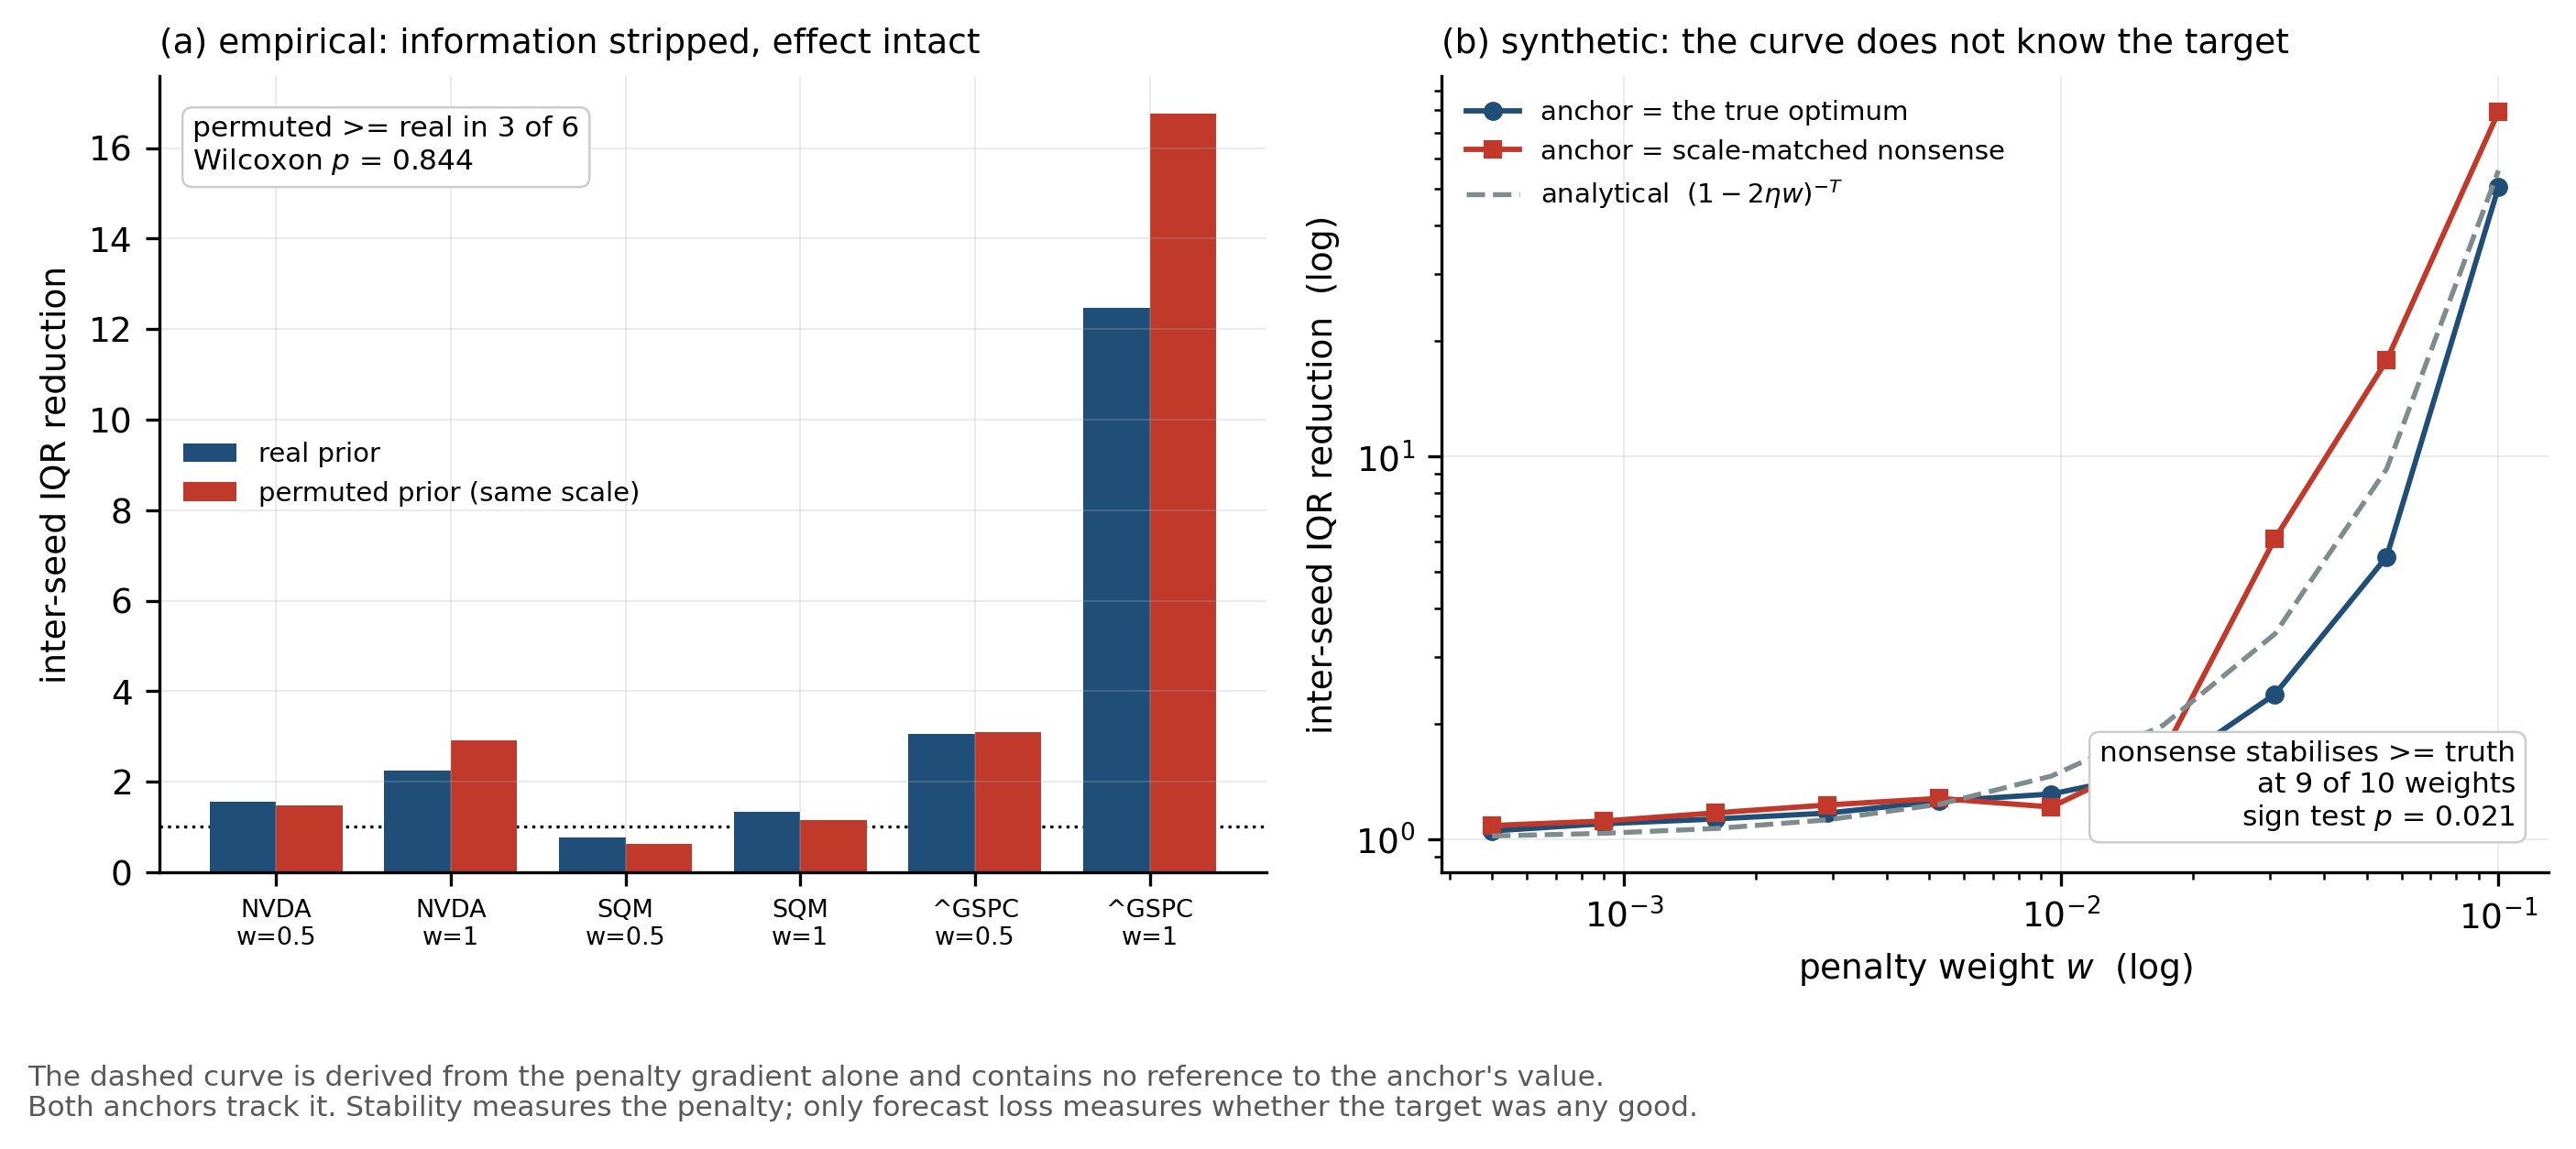
\includegraphics[width=\linewidth]{figures/figure2_control.png}\label{fig:control}
\caption{Figure 2}
\end{figure}

\textbf{Figure 2 is Figure 1 with a control.} Panel (a) repeats the empirical comparison against a
prior permuted in time; the effect is unchanged. Panel (b) overlays the analytical contraction
\texttt{(1\ $-$\ 2$\eta$w)\^{}$-$T} --- a curve derived from the penalty gradient alone, which contains no reference to
the anchor's value. Both the true and the nonsense anchor track it. The dashed line is the whole
argument: it predicts the data without knowing what the data was shrunk toward.

\begin{quote}
\textbf{This section was itself corrected twice, and both corrections are reported in \Cref{app:corrections}.}
An earlier version ran four weights and quoted the single most extreme cell; and the file this
draft reads its numbers from was later found to be stale, still holding the retracted values.
Neither changes the conclusion; both are the practice \Cref{sec:multiplicity} criticises, committed in our own
showcase.
\end{quote}

\textbf{The paired column above is the paper's central point.} Stability rises with the penalty for
any target; usefulness depends on the target being right. A study that reports the first as
evidence for the second has reported an identity.

\textbf{Generalisation.} For any regularised estimator, stability under a shrinkage penalty is not
evidence that the shrinkage target is good. The mechanism is Stein/ridge shrinkage and is not
itself new; what we document is that it is \textbf{reportable as an empirical finding}, that it
survives a pre-registered protocol with a dose--response and \(p = 5.2 \times 10^{-4}\), and that a
scale-matched permuted control detects it for minutes of compute.

\textbf{Nothing about that control is ours.} It is a restricted randomization test (Fisher 1935;
Pitman 1937; Ojala \& Garriga 2010), and the move it makes --- randomize the input a claim depends
on and check whether the claim survives --- is the move behind the random-label experiment of
Zhang et al.~(2017), the model- and data-randomization sanity checks of Adebayo et al.~(2018),
and the placebo laws of Bertrand, Duflo and Mullainathan (2004), who found conventional
difference-in-differences standard errors significant at 5\% for up to 45\% of interventions that
never happened. Four literatures already treat this as routine.

What we could not find is an instance applied to a \textbf{stability} claim rather than an accuracy
or treatment-effect claim. We state that as a search null and not as a gap: by the standard \Cref{sec:power}
applies to this study's own nulls, failing to find something is not evidence it is absent. We
offer \Cref{sec:tautology} as a template, not as a method --- and the appropriate conclusion is that a control
already standard in four fields should be applied in a fifth, which is a much weaker and much
more defensible claim than novelty.

\textbf{And the practice we set out to criticise turns out to be handled correctly where it
originates.} We expected to find regularisers proposed as remedies for run-to-run variance with
the resulting stability offered as evidence of quality. The first half is true: Bhojanapalli et
al.~(2021) propose exactly such regularisers. The second half is false --- they report accuracy
beside stability throughout, include a deterministic zero-variance control, and state our own
\Cref{sec:synthetic} point in prose (\Cref{app:survey}).

We report this because it weakens the section, and because it sharpens it. \textbf{Our error was not
reporting stability; it was inferring from stability a conclusion about the target.} Where
reduced run-to-run variance \emph{is} the objective, reporting it is correct. We instead used it as
evidence that the anchor carried risk information --- a claim about the target that no property of
the penalty can support.

The failure is therefore not a field's carelessness but what happens when a concept crosses
domains and its controls do not travel with it. The one documented instance of the inference
being made explicitly is a VaR paper (Petneházi 2019), offering \emph{``consistently lower standard
deviation than the benchmark methods\ldots{} which also justifies that this one produces the highest
quality VaR estimates''} with no matched control. We made the same move, in the same domain, four
years later.

\textbf{Every magnitude above carries a bootstrap interval.} The resampling unit is the
\emph{comparison}, because the quantity quoted is a median across comparisons. A seed-level interval
would answer a different question and requires the per-seed losses, which our pipeline did not
originally persist --- a gap we found only when trying to satisfy this requirement, and have since
closed. \textbf{The intervals are wide.} That is itself part of the finding: the magnitudes this
study reported were never as precise as a bare point estimate implies.
